\subsection{Administración de Configuración y Documentación}

El proyecto produce artefactos de varios tipos, código fuente, código de pruebas, documentación técnica, documentación académica y datos de configuración, que evolucionan a lo largo de los ciclos DSR. Para mantener trazabilidad, consistencia y la capacidad de retroceder a versiones anteriores si es necesario, se implementa un proceso riguroso de control de cambios.

Los ítems de configuración principales son identificados explícitamente. El código fuente del SDK en TypeScript (directorio src/) y el código de la API de simulación Fastify (directorio api/) se versionan en GitHub utilizando versionamiento semántico (MAJOR.MINOR.PATCH). Las pruebas unitarias (directorio test/) se mantienen sincronizadas con cambios en src/. La rama principal es main (código estable listo para publicación), la rama de desarrollo es dev (integración de nuevas features), y cada feature individual tiene su propia rama feature/nombre-descriptivo que se fusiona en dev una vez completada. La documentación técnica se almacena en docs/ en formato Markdown: architecture.md (descripción de patrones y componentes), sandbox-data.md (especificación de escenarios de prueba por pasarela), integration-guide.md (tutorial para desarrollador externo), y CHANGELOG.md (historial de cambios por versión). La documentación de APIs se genera automáticamente mediante TypeDoc cada build. La documentación académica (documento de trabajo de grado, reportes de fase) se almacena en Google Drive con historial de cambios y versionamiento manual (v0.1, v0.2, etc.). Los datos de configuración se mantienen en Google Sheets: plan de riesgos (Anexo B), plan de mitigación (Anexo C), y matriz de trazabilidad (sección 1.3).

Para cambios en código, se sigue un proceso estructurado: el desarrollador crea una rama feature/nombre-descriptivo, implementa el cambio localmente, ejecuta pruebas unitarias (jest --coverage) asegurando cobertura mínima del 80\%, pushea el código a GitHub, y crea una Pull Request (PR) describiendo brevemente el cambio. El CI/CD pipeline automático (GitHub Actions) compila el código, ejecuta pruebas, verifica coverage y ejecuta análisis de estilo (ESLint). Si hay errores, el desarrollador los corrige localmente e itera. Una vez que el build es exitoso, el Líder arquitectura y núcleo SDK y al menos otro integrante revisan el código verificando lógica correcta, aplicación de patrones de diseño GoF, y métricas de complejidad (WMC $\leq$15, CBO $\leq$5, RFC $\leq$20). Si la revisión identifica mejoras necesarias, se registran como comentarios en el PR; el desarrollador las aborda e itera. Una vez aprobado, se fusiona (merge) en la rama dev. Para cambios en documentación, el proceso es similar pero sin rama de feature: el autor modifica el documento en GitHub (si es .md) o Google Docs, otro integrante revisa verificando gramática, claridad y validez de referencias cruzadas, y una vez aprobado se considera finalizado. Al cierre de cada fase DSR (fin de H1, H2, etc.), se consolida la rama dev en main, se genera un tag de versión (ej. v0.1.0, v0.2.0), se publica la versión estable en npm, y se actualiza CHANGELOG.md con descripción de cambios incluidos.

La tabla de evolución de artefactos (Tabla en sección 7) define cuándo cada artefacto se crea, se refina, se expande, se optimiza, se publica o se archiva durante los hitos H1 a H6. Por ejemplo, el SDK src/ se crea en H1, se refina en H2, se expande en H3, se optimiza en H4, se finaliza en H5 y se publica en H6. La API de simulación se crea en H2, se expande en H3-H4, se despliega en H5 y se finaliza en H6. La documentación del trabajo de grado se comienza en H1 con un outline, se elaboran capítulos en cada fase posterior, y se entrega versión final en H6. Este cronograma asegura que todos los artefactos estén listos en el momento correcto y evolucionen gradualmente a lo largo del proyecto.

\begin{center}
\renewcommand{\arraystretch}{1.2}
\begin{longtable}{|P{0.243}|P{0.241}|P{0.241}|P{0.241}|}
  \hline
  \textbf{Artefacto} & \textbf{Ubicación} & \textbf{Tipo} & \textbf{Ciclo de vida (Hitos H1-H6)} \\
  \hline
  \endfirsthead
  \hline
  \textbf{Artefacto} & \textbf{Ubicación} & \textbf{Tipo} & \textbf{Ciclo de vida (Hitos H1-H6)} \\
  \hline
  \endhead
  \caption{Descripción de artefactos de documentación.}
  \label{tab:artefactos-documentacion}\\
  \endlastfoot
  SDK TypeScript \newline /src & GitHub (main/dev) & Código fuente & H1: Crear \newline H2: Refinar \newline H3: Expandir \newline H4: Optimizar \newline H5: Finalizar \newline H6: Publicar \\
  \hline
  Pruebas unitarias \newline /test & GitHub (main/dev) & Código de pruebas & H1: Crear \newline H2-H4: Expandir \newline H5: Mantener \newline H6: Auditar \\
  \hline
  API Fastify \newline /api & GitHub (main/dev & Código fuente & H2: Crear \newline H3-H4: Expandir \newline H5: Desplegar \newline H6: Finalizar \\
  \hline
  Documento de arquitectura \newline /docs/architecture.md & GitHub & Documentación técnica & H1: Crear \newline H2-H5: Refinar \newline H6: Publicar \\
  \hline
  Datos de prueba (sandbox) \newline /docs/sandbox-data.md & GitHub & Documentación técnica & H2: Crear \newline H3-H4: Expandir \newline H5: Consolidar \newline H6: Publicar \\
  \hline
  Guía de integración \newline /docs/integration-guide.md & GitHub & Documentación técnica & H3: Crear \newline H4-H5: Refinar \newline H6: Publicar \\
  \hline
  Registro de cambios \newline /CHANGELOG.md & GitHub & Documentación técnica & H1: Crear \newline H2-H5: Actualizar \newline H6: Consolidar \\
  \hline
  Documentación API (TypeDoc) \newline Generado automático & GitHub Pages & Documentación técnica & H1: Crear \newline H2-H5: Regenerar \newline H6: Publicar \\
  \hline
  Trabajo de grado \newline Documento final & Google Drive & Documentación académica & H1: Esbozo \newline H2-H4: Elaborar \newline H5: Revisar \newline H6: Entregar \\
  \hline
  Reportes de fase \newline Documento & Google Drive & Documentación académica & H1,H2,H3: Crear \newline H4,H5: Crear \newline H6: Crear \\
  \hline
  Matriz de trazabilidad \newline Google Sheets & Google Drive & Datos de configuración & H1: Crear \newline H2-H5: Actualizar \newline H6: Consolidar \\
  \hline
  Plan de riesgos \newline Anexo B & Google Sheets & Datos de configuración & H1: Crear \newline H2-H5: Mantener \newline H6: Archivar \\
  \hline
  Plan de mitigación \newline Anexo C & Google Sheets & Datos de configuración & H1: Crear \newline H2-H5: Mantener \newline H6: Archivar \\
  \hline
  Métricas de complejidad (CK) \newline Google Sheets & Google Drive & Datos de configuración & H2: Crear \newline H3-H5: Recolectar \newline H6: Reportar \\
  \hline
\end{longtable}
\end{center}

\begin{figure}[H]
  \centering
  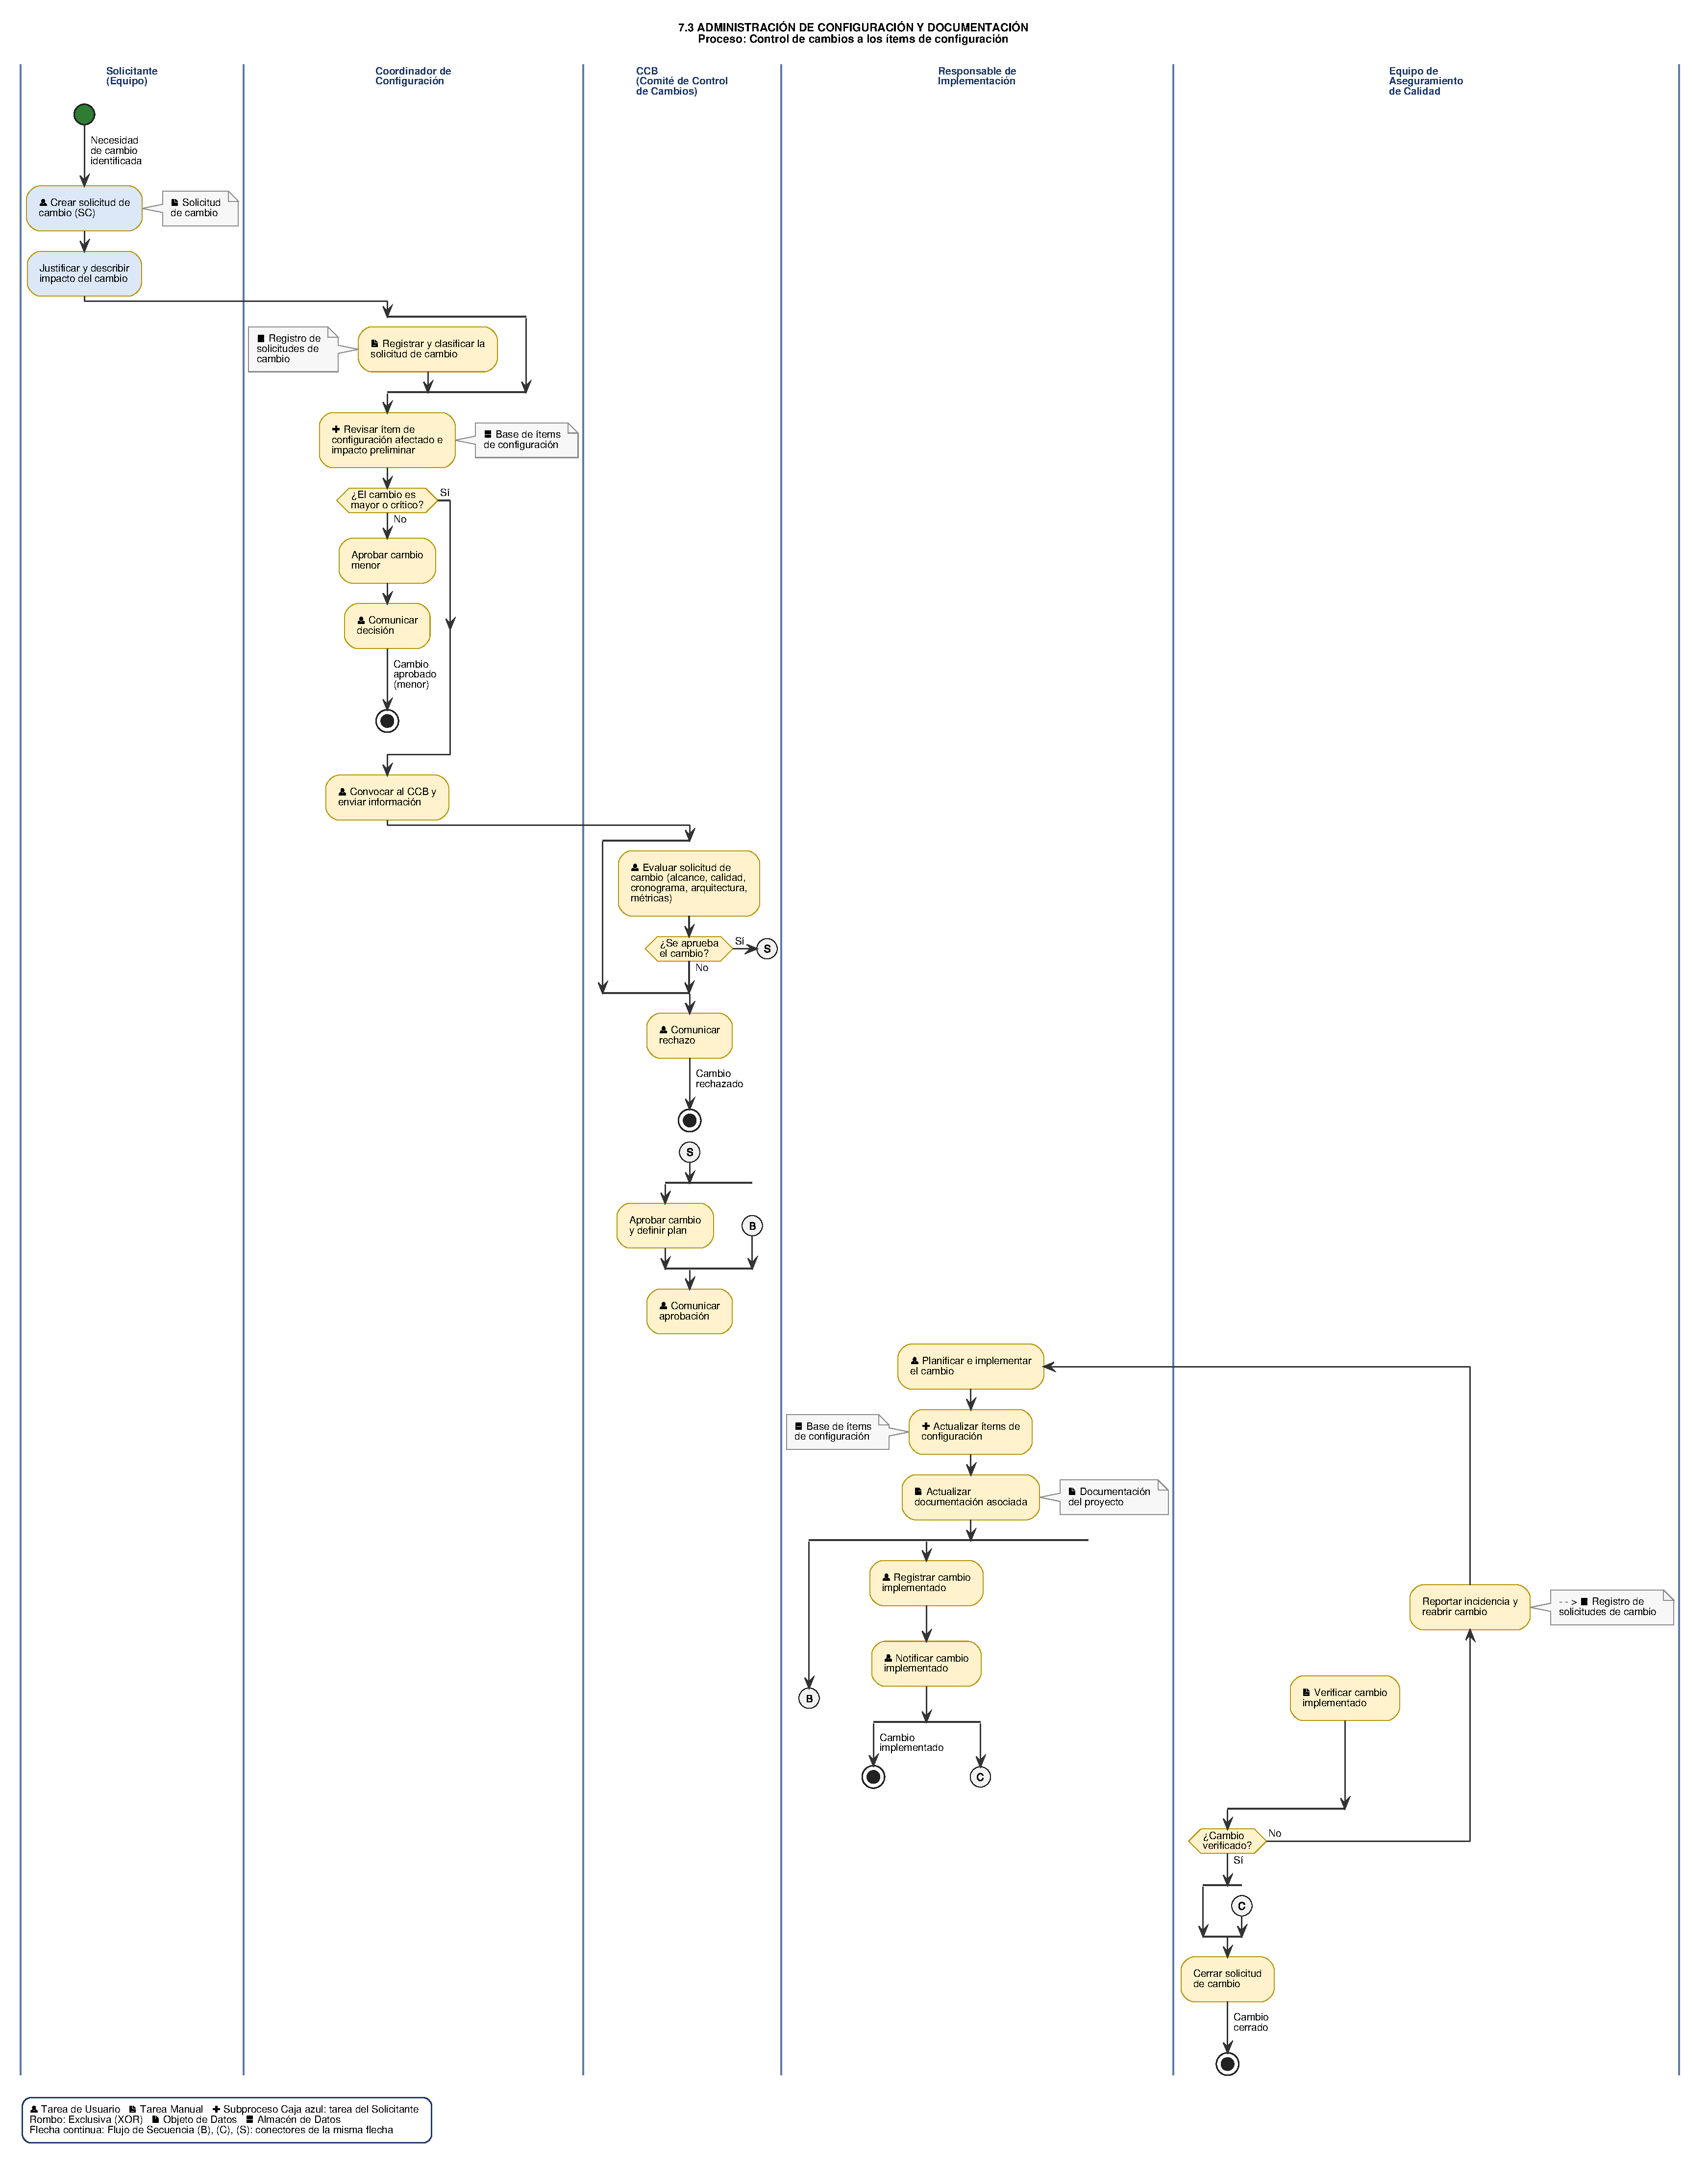
\includegraphics[width=\textwidth]{figuras/07-bpmn-documentacion}
  \caption{Diagrama BPMN para documentación}
  \label{fig:bpmn-documentacion}
\end{figure}
